%6_Poisson_distribution.tex

%notes for the course Mathematics for Computer Scientists A
%taught at the University of Bristol
%2020_21 Conor Houghton conor.houghton@bristol.ac.uk

%To the extent possible under law, the author has dedicated all copyright 
%and related and neighboring rights to these notes to the public domain 
%worldwide. These notes are distributed without any warranty. 


\documentclass[11pt,a4paper]{scrartcl}
\typearea{12}
\usepackage{graphicx}
%\usepackage{pstricks}
\usepackage{listings}
\usepackage{color}


\newif\ifind
\indtrue


\lstset{language=C}
\usepackage{fancyhdr}
\pagestyle{fancy}
\lfoot{\texttt{cs-uob.github.io/COMS10014/}}
\rfoot{\texttt{coms10011.github.io}}
\lhead{COMS10014 Poisson Distribution - Conor}
\begin{document}

\section*{6 Poisson distribution}

Imagine someone fishing in a large lake; say the lake is so large that
catching one fish doesn't effect the chance they'll catch
another. Imagine too that the fishing conditions don't change
day-by-day or hour-by-hour. Say we know how many fish they catch on
average an hour, say five, but we want to estimate the probability
that they catch four. In other words we know the average rate they
catch fish, but the actual event, the fish chancing upon the lure and
getting hooked, is random, and we want to know the distribution of this
event count over an interval. This distribution is an example of the
Poisson distribution and is the subject of this section.\footnote{This
  joke, pretending the Poisson distribution is so named because it is
  related to fish, rather than because it is named after the
  mathematician Sim\'{e}on Denis Poisson, I stole from Eddie Wilson in
  Engineering Mathematics. Poisson wrote about the Poisson
  distribution in a book about how to estimate the number of wrongful
  convictions; the distribution became well known after Ladislaus
  Bortkiewicz used it in an investigation of how many Prussian
  soldiers each year were killed by horse kicks. Both these examples
  are like the fishing example, you want to study the relationship
  between the rate of something happening and the distribution of
  different numbers of occurrences.}

\subsection*{Deriving the Poisson distribution}

The Poisson distribution can be derived from the bionomial
distribution, it just requires a nerve-wracking limit. Imagine slicing
time up into small slices, each so small there is a vanishingly small
chance of two events happening and that the chance of one event is
$p$. Thus, $P(\mbox{one fish})=p$, $P(\mbox{no fishes})=1-p$ and
$P(\mbox{more than one fishes})=0$. Of course this is nonsense, if
there can be one fish there is some chance of two, but we are going to
take the limit where the time interval becomes zero so this doesn't
matter. Call the small interval width $\delta t$.


\begin{figure}[tb]
\begin{center}
% GNUPLOT: LaTeX picture with Postscript
\begingroup
  \makeatletter
  \providecommand\color[2][]{%
    \GenericError{(gnuplot) \space\space\space\@spaces}{%
      Package color not loaded in conjunction with
      terminal option `colourtext'%
    }{See the gnuplot documentation for explanation.%
    }{Either use 'blacktext' in gnuplot or load the package
      color.sty in LaTeX.}%
    \renewcommand\color[2][]{}%
  }%
  \providecommand\includegraphics[2][]{%
    \GenericError{(gnuplot) \space\space\space\@spaces}{%
      Package graphicx or graphics not loaded%
    }{See the gnuplot documentation for explanation.%
    }{The gnuplot epslatex terminal needs graphicx.sty or graphics.sty.}%
    \renewcommand\includegraphics[2][]{}%
  }%
  \providecommand\rotatebox[2]{#2}%
  \@ifundefined{ifGPcolor}{%
    \newif\ifGPcolor
    \GPcolorfalse
  }{}%
  \@ifundefined{ifGPblacktext}{%
    \newif\ifGPblacktext
    \GPblacktexttrue
  }{}%
  % define a \g@addto@macro without @ in the name:
  \let\gplgaddtomacro\g@addto@macro
  % define empty templates for all commands taking text:
  \gdef\gplbacktext{}%
  \gdef\gplfronttext{}%
  \makeatother
  \ifGPblacktext
    % no textcolor at all
    \def\colorrgb#1{}%
    \def\colorgray#1{}%
  \else
    % gray or color?
    \ifGPcolor
      \def\colorrgb#1{\color[rgb]{#1}}%
      \def\colorgray#1{\color[gray]{#1}}%
      \expandafter\def\csname LTw\endcsname{\color{white}}%
      \expandafter\def\csname LTb\endcsname{\color{black}}%
      \expandafter\def\csname LTa\endcsname{\color{black}}%
      \expandafter\def\csname LT0\endcsname{\color[rgb]{1,0,0}}%
      \expandafter\def\csname LT1\endcsname{\color[rgb]{0,1,0}}%
      \expandafter\def\csname LT2\endcsname{\color[rgb]{0,0,1}}%
      \expandafter\def\csname LT3\endcsname{\color[rgb]{1,0,1}}%
      \expandafter\def\csname LT4\endcsname{\color[rgb]{0,1,1}}%
      \expandafter\def\csname LT5\endcsname{\color[rgb]{1,1,0}}%
      \expandafter\def\csname LT6\endcsname{\color[rgb]{0,0,0}}%
      \expandafter\def\csname LT7\endcsname{\color[rgb]{1,0.3,0}}%
      \expandafter\def\csname LT8\endcsname{\color[rgb]{0.5,0.5,0.5}}%
    \else
      % gray
      \def\colorrgb#1{\color{black}}%
      \def\colorgray#1{\color[gray]{#1}}%
      \expandafter\def\csname LTw\endcsname{\color{white}}%
      \expandafter\def\csname LTb\endcsname{\color{black}}%
      \expandafter\def\csname LTa\endcsname{\color{black}}%
      \expandafter\def\csname LT0\endcsname{\color{black}}%
      \expandafter\def\csname LT1\endcsname{\color{black}}%
      \expandafter\def\csname LT2\endcsname{\color{black}}%
      \expandafter\def\csname LT3\endcsname{\color{black}}%
      \expandafter\def\csname LT4\endcsname{\color{black}}%
      \expandafter\def\csname LT5\endcsname{\color{black}}%
      \expandafter\def\csname LT6\endcsname{\color{black}}%
      \expandafter\def\csname LT7\endcsname{\color{black}}%
      \expandafter\def\csname LT8\endcsname{\color{black}}%
    \fi
  \fi
  \setlength{\unitlength}{0.0500bp}%
  \begin{picture}(5040.00,3528.00)%
    \gplgaddtomacro\gplbacktext{%
      \csname LTb\endcsname%
      \put(858,679){\makebox(0,0)[r]{\strut{} 0}}%
      \put(858,1110){\makebox(0,0)[r]{\strut{} 0.05}}%
      \put(858,1540){\makebox(0,0)[r]{\strut{} 0.1}}%
      \put(858,1971){\makebox(0,0)[r]{\strut{} 0.15}}%
      \put(858,2402){\makebox(0,0)[r]{\strut{} 0.2}}%
      \put(858,2832){\makebox(0,0)[r]{\strut{} 0.25}}%
      \put(858,3263){\makebox(0,0)[r]{\strut{} 0.3}}%
      \put(1050,484){\rotatebox{-270}{\makebox(0,0)[r]{\strut{} 0}}}%
      \put(1649,484){\rotatebox{-270}{\makebox(0,0)[r]{\strut{} 5}}}%
      \put(2248,484){\rotatebox{-270}{\makebox(0,0)[r]{\strut{} 10}}}%
      \put(2846,484){\rotatebox{-270}{\makebox(0,0)[r]{\strut{} 15}}}%
      \put(3445,484){\rotatebox{-270}{\makebox(0,0)[r]{\strut{} 20}}}%
      \put(4044,484){\rotatebox{-270}{\makebox(0,0)[r]{\strut{} 25}}}%
      \put(4643,484){\rotatebox{-270}{\makebox(0,0)[r]{\strut{} 30}}}%
    }%
    \gplgaddtomacro\gplfronttext{%
      \csname LTb\endcsname%
      \put(3656,3090){\makebox(0,0)[r]{\strut{}$\lambda=2$}}%
      \csname LTb\endcsname%
      \put(3656,2870){\makebox(0,0)[r]{\strut{}$\lambda=10$}}%
      \csname LTb\endcsname%
      \put(3656,2650){\makebox(0,0)[r]{\strut{}$\lambda=20$}}%
    }%
    \gplbacktext
    \put(0,0){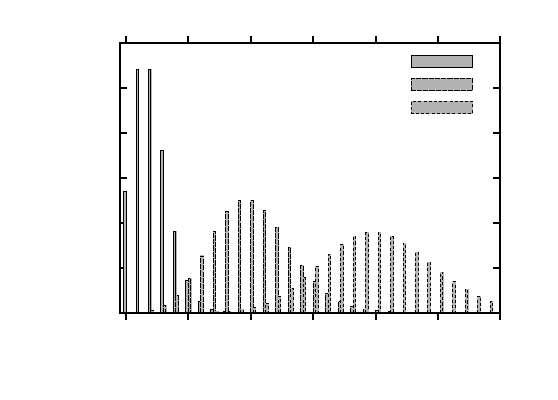
\includegraphics{fig_dist}}%
    \gplfronttext
  \end{picture}%
\endgroup

\end{center}
\caption{The Poisson distribution for a variety of values of $\lambda$. As $\lambda$ increases the peak moves to the right.\label{fig_dist}}
\end{figure}


Now if we are interested in the probability distribution for the
number of events in an interval $T=n\delta t$, then, by the binomial
distribution the probability of $r$ events is
\begin{equation}
p(r)=\left(\begin{array}{c}n\\r\end{array}\right)p^r(1-p)^{n-r}
\end{equation}
Now write $\delta t=T/n$ and consider the $n\rightarrow \infty$ limit:
\begin{equation}
p(r)=\lim_{n\rightarrow\infty}\left(\begin{array}{c}n\\r\end{array}\right)p^r(1-p)^{n-r}
\end{equation}
Since $p$ is the probability of an event in the small interval, it
will become tiny as $n$ becomes large, so, to deal with quantities
that remain useful in the limit, let $\lambda=np$. Substituting this
in, and expanding out the binomial coefficient:
\begin{equation}
p(r)=\lim_{n\rightarrow\infty}\frac{n(n-1)(n-2)\ldots (n-r+1)}{r!}\left(\frac{\lambda}{n}\right)^r\left(1-\frac{\lambda}{n}\right)^{n-r}
\end{equation}
As $n$ gets large the numerator of the first fraction just looks like $n^r$ and cancels with the denominator of the second fraction. Recall that
\begin{equation}
\lim_{n\rightarrow \infty}\left(1-\frac{x}{n}\right)^n=e^{-x}
\end{equation}
The $(1-\lambda/n)^{n-r}$ term has an extra $-r$ but
\begin{equation}
\lim_{n\rightarrow \infty}\left(1-\frac{\lambda}{n}\right)^{-r}=1
\end{equation}
Putting all this together we get
\begin{equation}
p(r)=\frac{\lambda^r}{r!}e^{-\lambda}
\end{equation}

First, it is easy to check that the probabilities add to one; but
notice that this range of the random variable is infinite!  Using the
Taylor expansion of the exponential:
\begin{equation}
e^x=\sum_{r=0}^\infty \frac{x^r}{r!}
\end{equation}
we have
\begin{equation}
\sum_{r=0}^\infty \frac{\lambda^r}{r!}e^{-\lambda}=e^{-\lambda}\sum_{r=0}^\infty \frac{\lambda^r}{r!}=e^{-\lambda}e^{\lambda}=1
\end{equation}
Next consider the mean
\begin{equation}
\mu = \sum_{r=0}^\infty r\frac{\lambda^r}{r!}e^{-\lambda}
\end{equation}
Because of the $r$ in the summand, the $r=0$ term is zero, so
\begin{equation}
\mu = \sum_{r=1}^\infty r\frac{\lambda^n}{r!}e^{-\lambda}
\end{equation}
Now, use $r!=r\times (r-1)!$:
\begin{equation}
  \mu = \sum_{r=1}^\infty \frac{\lambda^r}{(r-1)!}e^{-\lambda}
\end{equation}
and then pull a $\lambda$ out the front
\begin{equation}
\mu = \lambda \sum_{r=1}^\infty \frac{\lambda^{r-1}}{(r-1)!}e^{-\lambda}
\end{equation}
Finally set $s=r-1$ and
\begin{equation}
\mu = \lambda \sum_{s=0}^\infty \frac{\lambda^s}{s!}e^{-\lambda}=\lambda
\end{equation}
so $\lambda$ is the average event count!

This calculation can also be done using the same approach we used for the binomial distribution: by differenciating
\begin{equation}
  Z=\sum_{r=0}^\infty p(r)=1
\end{equation}
In this case
\begin{equation}
  0=\frac{d}{d\lambda}Z=\frac{d}{d\lambda}\sum_{r=0}^\infty \frac{\lambda^r}{r!}e^{-\lambda}
\end{equation}
Using the product rule
\begin{equation}
0= \sum_{r=0}^\infty \frac{r\lambda^{r-1}}{r!}e^{-\lambda}-\sum_{r=0}^\infty \frac{\lambda^r}{r!}e^{-\lambda}
\end{equation}
Now the second term is just $Z$ again, that is one, then multiplying and dividing by $\lambda$ in the first term gives
\begin{equation}
  0=\frac{1}{\lambda}\sum_{r=0}^\infty \frac{r\lambda^r}{r!}e^{-\lambda}-1
\end{equation}
Noting the first sum is just the average we get
\begin{equation}
  \mu=\lambda
\end{equation}
as before. This same method could be used to derive the variance.

Some example Poisson distributions are shown in Fig.~\ref{fig_dist}.

\subsection*{Quick example}

An average of two supervillians arrive at Gotham every day; Batman has
little trouble fighting them off, in fact he can fight off six
supervillians a day. Seven would be tricky though. What is the chance
seven supervillians arrive in one day?
\begin{equation}
p(7)=\frac{2^7}{7!}e^{-2}\approx 0.0034
\end{equation}
so makes it seem Batman will probably be ok, however, you should note
there are 365 days in the year. As for the fishing example:
\begin{equation}
p(4)=\frac{5^4}{4!}e^{-5}\approx 0.19
\end{equation}

\ifind
\section*{Summary}
\else
\subsection*{9 Gauss distribution}
\fi

\begin{itemize}

\item The \textbf{Gau\ss{}ian distribution} has density
  \begin{equation}
p(x)=\frac{1}{\sqrt{2\pi\sigma^2}}e^{-\frac{(x-\mu)^2}{2\sigma^2}}
  \end{equation}


\item You can  shown that the mean is $\mu$ and the variance is $\sigma^2$ as the notation would suggest by differenciating
\begin{equation}
1=Z=\int_{-\infty}^\infty p(x)dx
\end{equation}
with respect to $\mu$.

%\item It has moment generating function
%  \begin{equation}
%m(t)= e^{\mu t + \frac{1}{2}\sigma^2 t^2}
%  \end{equation}
%  from which can be be shown that the mean is $\mu$ and the variance is $\sigma%^2$ as the notation would suggest.

\item To work out probabilities you need to use the \textbf{error function}
  \begin{equation}
\mbox{erf}\,(x)=\frac{1}{\sqrt{\pi}}\int_{-x}^xe^{-y^2}dy=\frac{2}{\sqrt{\pi}}\int_0^xe^{-y^2}dy
  \end{equation}
  In fact
  \begin{equation}
\mbox{Prob}(x_1<x<x_2)=\frac{1}{2}[\mbox{erf}\,(z_2)-\mbox{erf}\,(z_1)]
  \end{equation}
  where
  \begin{equation}
z=\frac{x-\mu}{\sqrt{2}\sigma}
  \end{equation}
  \end{itemize}


\ifind
\section*{Example question}
\else
\subsection*{2 conditional probability - example question}
\fi

This is known as the `second sibling' problem and like the Monty Hall problem it was popularized by Marilyn Vos Savant:
\begin{quote}
 A shopkeeper says she has two new baby beagles to show you, but
    she doesn't know whether they're male, female, or a pair. You tell
    her that you want only a male, and she telephones the fellow who's
    giving them a bath. "Is at least one a male?" she asks him. "Yes!"
    she informs you with a smile. What is the probability that the
    other one is a male?
\end{quote}

\noindent \textbf{solution} So we are assuming that males and females are equally likely and that the sex of the two pups is independent; the set of outcomes, using the obvious notation, is $\mathcal{X}=\{(m,m),(m,f),(f,m),(f,f)\}$ with each event having probability $1/4$. The event that at least one is male is $\mathcal{M}=\{(m,m),(m,f),(f,m)\}$. This means that $P(\mathcal{M})=3/4$. Lets call the event that the second dog is male $\mathcal{S}$ so $\mathcal{M}\cap\mathcal{S}=\{(m,m)\}$ and
\begin{equation}
P(\mathcal{M}\cap\mathcal{S})=\frac{1}{4}
\end{equation}
and hence
\begin{equation}
P(\mathcal{S}|\mathcal{M})=\frac{1}{3}
\end{equation}
and so the probability the second dog is male is one in three.



\end{document}




